\NeedsTeXFormat{LaTeX2e}
%\PassOptionsToClass{handout}{beamer}
\documentclass{beamer}
\usepackage{beamerPack}
\usepackage{amsmath}
\usepackage{setspace}
\usepackage[07]{../lecture}
\subtitle{データ構造とアルゴリズム}
\begin{document}

\begin{frame}[fragile]{}
\titlepage
\end{frame}

\section{Hash Table}		%%%%%%%%
\subsection{}

\begin{frame}[fragile]{ハッシュ表}{検索の高速化}

検索アルゴリズム(配列は値を保持):
\[
キー \stackrel{O(\log(n))}{\longrightarrow} 配列中の値
\]

\vfill
ハッシュ表(配列は値が存在するかしないかを保持):
\[
キー \stackrel{O(1)}{\longrightarrow} 添字 \stackrel{O(1)}{\longrightarrow} 配列[添字]
\]

\vfill
キーから添字への変換関数をハッシュ関数という。
\end{frame}

\begin{frame}[fragile]{ハッシュ関数の例}{}
氏名(\texttt{name})からの顧客情報の獲得(最大文字数は10とする)

\begin{align*}
添字
&= \text{name}[0]の文字コード\times \text{存在する文字数}^{9}\\
&+ \text{name}[1]の文字コード\times \text{存在する文字数}^{8}\\
& \cdots \\ 
&+ \text{name}[9]の文字コード\times \text{存在する文字数}^{0}\\
\end{align*}

必要な配列の大きさは文字コードを固定長4Byte$=2^{32}$として$2^{320}$程度。
顧客数に関わらずこの計算は乗算10回加算10回で$O(1)$。
\end{frame}

\begin{frame}[fragile]{ハッシュについて}{}
\begin{itemize}\itemsep8pt
\item ハッシュ値の衝突
\begin{itemize}\itemsep8pt
\item リストを使う
\item 隣を使う
\end{itemize}
\item 挿入、削除、検索全て$O(1)$だが用途によっては注意(巡回が遅かった)
\item P2Pでは分散ハッシュテーブル(DHT)を多用
\end{itemize}
\end{frame}

\section{Heap}		%%%%%%%%
\subsection{}

\begin{frame}[fragile]{ヒープ}{}

親の値が子の値よりも常に$\le$(または$\ge$)になっている木(特に二分木)。

\begin{enumerate}\itemsep8pt
\item 要素の追加、先頭要素の削除の手間が$O(\log(N))$
\item 配列で実現できる
\end{enumerate}
\end{frame}


\begin{frame}[fragile]{ヒープの操作}{}
要素の追加

\begin{enumerate}%\itemsep8pt
\item 末尾に追加する
\item 親と比べて$\ge$(または$\le$)なら親と入れ替え。この操作を再帰的に実行(高さが$O(\log(n))$)
\end{enumerate}

先頭要素の削除
\begin{enumerate}%\itemsep8pt
\item 先頭がなくなるので、末尾の要素を先頭に持ってくる
\item 直下の二つの子との関係がおかしくなるので入れ替える(どちらと?)。この操作を再帰的に実行。
\end{enumerate}

動的に要素が追加される状況で常に最小値(最大値)を$O(\log(n))$で取り出せるので整列、検索の組み合わせよりも高速。OSのプロセススケジューリングが代表例。
\end{frame}

\begin{frame}[fragile]{ヒープは配列に埋め込める}{wikipediaと比較}

\begin{center}
\scalebox{0.6}{
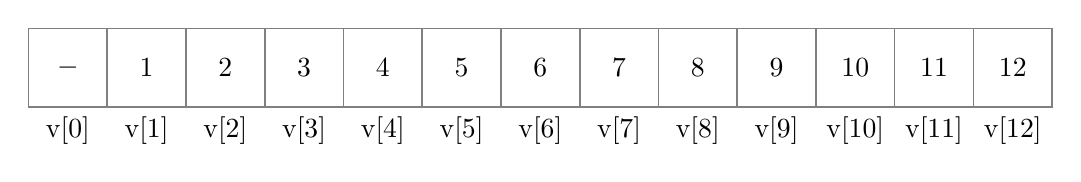
\begin{tikzpicture}[
    , cell/.style = {rectangle,draw=gray,semithick,minimum size=1cm,outer sep = 0mm,label=below:v{[\j]}}
]
\foreach \i [count=\j from 0] in {-, 1, 2, 3, 4, 5, 6, 7, 8, 9, 10, 11, 12}
    \node[cell] at (\j, 0) {$\i$};
\end{tikzpicture}
}
\end{center}
\texttt{v[0]}は使わない

\vfill
\begin{itemize}%\itemsep8pt
\item \texttt{v[i]}から見た左の子: \texttt{v[2*i]}
\item \texttt{v[i]}から見た右の子: \texttt{v[2*i + 1]}
\item \texttt{v[i]}から見た親: \texttt{v[i/2]}
\end{itemize}
\end{frame}

\section{Graph}		%%%%%%%%
\subsection{}

\begin{frame}[fragile]{グラフ}{一般のグラフをどうやって計算機上に表現するか}
\begin{itemize}%\itemsep8pt
\item 木ならJSONでもいいが、グラフ(合流、逆戻りあり)をどうやって表現するのか
\item 特に特徴量の計算が必要な場合、ポインタを使うのが正解とは限らない
\end{itemize}

配列表現の例
\begin{center}
\begin{tabular}{|r| l | l |}
\hline
添字 & 値 & 添字の集合 \\\hline
0 & "abc" & [1, 2] \\\hline
1 & "xyz" & [] \\\hline
2 & "def" & [3] \\\hline
3 & "cba" & [0] \\\hline
\end{tabular}
\end{center}

\begin{itemize}%\itemsep8pt
\item オブジェクト "abc" (id = 0) は1と2と直接関係
\item オブジェクト "def" (id = 2) は3と直接関係
\item オブジェクト "cdb" (id = 3) は0と直接関係
\end{itemize}
\end{frame}

\begin{frame}[fragile]{配列表現されたグラフ上の計算例}{}
\begin{columns}
\begin{column}{0.5\textwidth}
\begin{itemize}%\itemsep8pt
\item 0は1と2と関係
\item 2は3と直接関係
\item 3は0と直接関係
\end{itemize}
\end{column}
\begin{column}{0.5\textwidth}
\[
\tilde{A} = 
\begin{pmatrix}
0 & 1 & 1 & 0\\
0 & 0 & 0 & 0\\
0 & 0 & 0 & 1\\
1 & 0 & 0 & 0\\
\end{pmatrix}
\]
\end{column}
\end{columns}
\vfill
対称性がある(無向グラフ)なら対称行列にすればよい
\vfill
\begin{columns}
\begin{column}{0.5\textwidth}
\begin{itemize}%\itemsep8pt
\item 自分は自分と関係がある
\end{itemize}
\end{column}
\begin{column}{0.5\textwidth}
\[
A^{1} = 
\begin{pmatrix}
1 & 1 & 1 & 0\\
0 & 1 & 0 & 0\\
0 & 0 & 1 & 1\\
1 & 0 & 0 & 1\\
\end{pmatrix}
\]
\end{column}
\end{columns}
\end{frame}

\begin{frame}[fragile]{行列による関係性の表現}{}
$A^2$: 友達の友達は友達: $i\to j \wedge j \to k$なら$i \to k$

\[
A^{2} = A^{1}A^{1} = 
\begin{pmatrix}
1 & 1 & 1 & 0\\
0 & 1 & 0 & 0\\
0 & 0 & 1 & 1\\
1 & 0 & 0 & 1\\
\end{pmatrix}
\begin{pmatrix}
1 & 1 & 1 & 0\\
0 & 1 & 0 & 0\\
0 & 0 & 1 & 1\\
1 & 0 & 1 & 1\\
\end{pmatrix}
=
\begin{pmatrix}
2 & 2 & 2 & 1\\
0 & 1 & 0 & 0\\
1 & 0 & 1 & 1\\
1 & 0 & 2 & 1\\
\end{pmatrix}
\]

$A^3$: 友達の友達の友達は友達

\[
A^{3} = A^{1}A^{2} = 
\begin{pmatrix}
1 & 1 & 1 & 0\\
0 & 1 & 0 & 0\\
0 & 0 & 1 & 1\\
1 & 0 & 0 & 1\\
\end{pmatrix}
\begin{pmatrix}
1 & 1 & 1 & 1\\
0 & 1 & 0 & 0\\
1 & 0 & 1 & 1\\
1 & 0 & 1 & 1\\
\end{pmatrix}
=
\begin{pmatrix}
3 & 2 & 3 & 3\\
0 & 1 & 0 & 0\\
3 & 0 & 3 & 3\\
3 & 0 & 3 & 3\\
\end{pmatrix}
\]
\end{frame}

\begin{frame}[fragile]{行列計算による関係の計算}{}
\begin{columns}
\begin{column}{0.5\textwidth}
\begin{itemize}%\itemsep8pt
\item 0は1と10.5 DM/day
\item 0は2と1.0 DM/day
\item 0は3と0.2 DM/day
\item 1は0と10.6 DM/day
\item 1は2と0.0 DM/day
\end{itemize}
\end{column}
\begin{column}{0.5\textwidth}
\[
R = 
\begin{pmatrix}
0 & 10.5 & 1.0 & 0.2 & \cdots \\
10.6 & 0 & 0.0 & ? & \cdots\\
? & ? & 0 & ? & \cdots\\
? & ? & ? & 0 & \cdots \\
\cdots & \cdots & \cdots & \cdots & \cdots\\
\end{pmatrix}
\]
\end{column}
\end{columns}

\vfill
\[
RR = R^{2} \to RR^{2} = R^{3} \to RR^{3} = R^{4} \cdots \longrightarrow R^{\infty}
\]

(適切な正規化をすることでこの計算は不動点を持つ)

\vfill
$R^{\infty}$:全ユーザの関係性; TL構築、recommendationの基本
\vfill
そしてもちろん行列は配列で実装できる
\end{frame}

\begin{frame}[fragile]{グラフと木関連}{配列ではなく木を対象にした探索}

一般にゲームなどで状態に応じて次の局面が決まるような問題は木になるので、最善手を
「考える」ことは木の中での最大値の「探索」に対応する。二分探索は配列に埋め込まれた(よい性質を持つ)二分木上の探索。

\begin{exampleblock}{深さ優先探索; Depth First Search(DFS)}
再帰的に探索。再帰関数で実装すると自然にこの探索になる。
\end{exampleblock}

\begin{exampleblock}{幅優先探索; Breath First Search(BFS)}
根に近い(浅い)ところから探索。探索すべき点をキューを使って管理。
\end{exampleblock}
ダイクストラ法は浅いではなく近いという点が少し違う。
\end{frame}

\begin{frame}[fragile]{グラフと木関連}{ヒューリスティック探索}
ゲームの木は大変に大きいので最良値探索は非現実的:近似解

\begin{exampleblock}{$A^{*}$探索}
これまでのコスト(厳密に計算)+これから予想されるコスト(近似計算)で距離を定めるダイクストラ法
\end{exampleblock}

\begin{exampleblock}{モンテカルロ木探索}
どの方向に探索を進めるかをモンテカルロ法で決定する。
\end{exampleblock}

\begin{exampleblock}{焼きなまし法; Simulated Annealing}
よさそうな点の回りを集中的に探索すると局所解に陥る可能性があるので、時々違う点の探索に移る。
どれだけの頻度、距離のジャンプを行うかを熱を模した変数で制御。
\end{exampleblock}

Min-Max法も名前だけ列挙。
\end{frame}

\begin{frame}[fragile]{グラフと木関連}{その他}
\begin{exampleblock}{トポロジカルソート}
有向非巡回グラフ(合流があるので木ではない)の整列アルゴリズム。
多重継承OOPLにおけるメソッド呼び出しが代表例。
\end{exampleblock}

\begin{exampleblock}{最小全域木}
全域木(グラフを全てカバーする木)の中で最小コストのものを構成する問題。
コンピュータネットワークの経路構築の基本。
\end{exampleblock}

\begin{exampleblock}{組合せ爆発: Combinatorial explosion}
データの大きさ$N$に対して計算時間が階乗的または指数関数的に増える状況。
\end{exampleblock}
{
\fontsize{6}{6}\selectfont
$N^3$, $N^4$, $N^{100}$などは指数関数ではないので組合せ爆発と言いたくないのだが、言うこともあるらしい。それらはたかだか多項式なのでP。NPなものを要求するなら指数的爆発と言った方がいいようだ。
}
\end{frame}

\end{document}
